\chapter{Embedded Systems Overview and Key Concepts}

\section{Definition of Embedded System}

% Embedded System are computing  system with \textbf{strongly coupled} hardware and software integration, designed to perform a \textbf{dedicate functionality}


\begin{tcolorbox}[colback=blue!5!white, colframe=blue!50!white, arc=0mm, sharp corners]

% \begin{center}
%     \textbf{\Large CIA triad \Large}\\
% \end{center}
Embedded System are computing  system with \textbf{strongly coupled} hardware and software integration, designed to perform a \textbf{dedicate functionality.}
\end{tcolorbox}
\paragraph{}

The world \textbf{embedded} means: build into, to be an integral part of, a large system.


The larger system is called \textbf{Embedding System}.

\begin{figure}[H]
    \centering
    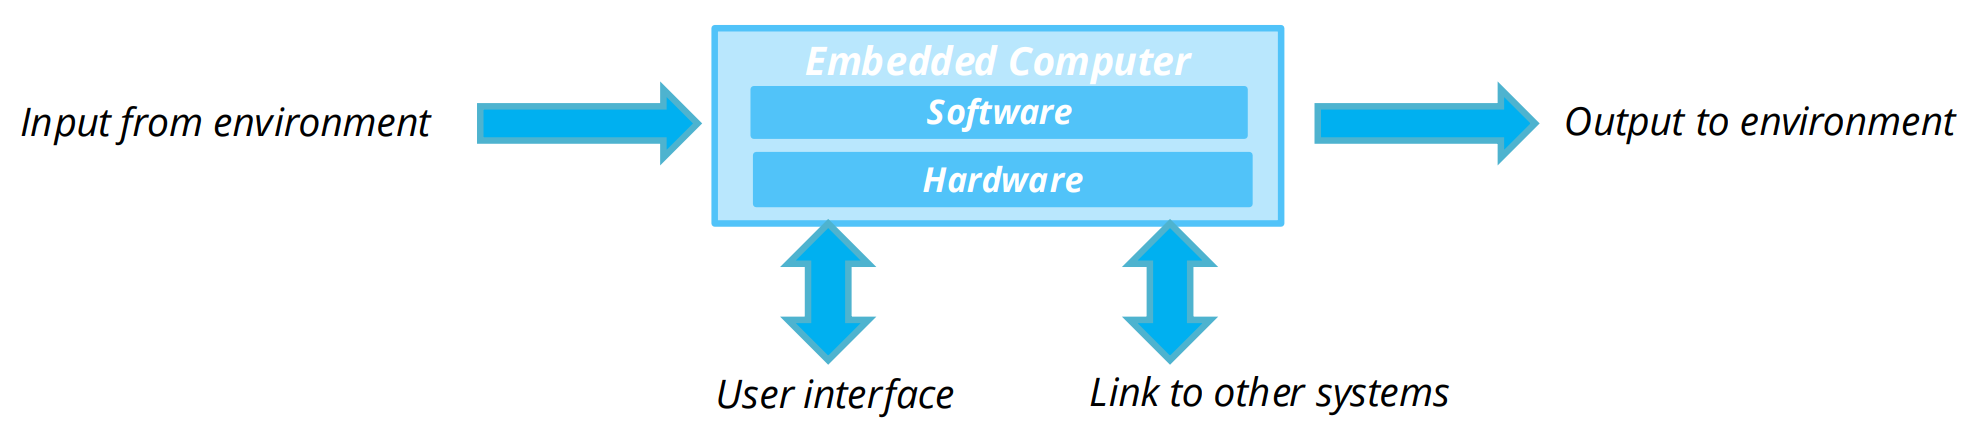
\includegraphics[width=0.8\linewidth]{img/img1.png}
    \caption{Embedded Computer}
\end{figure}

Another definition of embedded system: 

\begin{tcolorbox}[colback=blue!5!white, colframe=blue!50!white, arc=0mm, sharp corners]
\textbf{Application-specific} computer system often with \textbf{real-time computer constraints}.
Implemented using \textbf{MCUs}, MicroControllerUnit.
\end{tcolorbox}

\paragraph{}
Embedded systems are added to larger system for different reasons:

\begin{itemize}
    \item Lower cost;
    \item Lower performance;
    \item Energy efficiency;
    \item More Functions and Features.
\end{itemize}

\newpage
\subsection{Example of some Embedded Systems}

\paragraph{Bike Computer}

\begin{itemize}
    \item Functions: speed and distance measurements;
    \item Constraints: size, cost, power and energy, weight;
    \item Inputs: wheel rotation that indicate how fast we are;
    \item Output: Display the speed;
    \item Use Low-Performance Microcontroller: 8-bit, 10 MIPS.
\end{itemize}

We can see that all the constraint change the design, software and hardware integration.

\paragraph{Automotive Embedded System}

Nowadays, cars are fully of microprocessors that detect different events that occur while driving or not:

\begin{itemize}
    \item 4-bit microcontroller checks seat belts;
    \item Microcontrollers run dashboard device;
    \item 16/32-bit microprocessor controls the engine...
\end{itemize}


\section{Microprocessor VS Microcontroller}

What is the difference between  \textbf{Microprocessor}, CPU, and\textbf{Microcontroller}, MCU?


Both have a \textbf{CPU core} to execute instructions.

\subsection{Microprocessor, CPU}

The \textbf{microprocessor (CPU) is a single core processor} that support at least the instruction of \textit{fetching}, \textit{decoding} and \textit{executing}. 

Normally it is used for a general purpose computer, it also \textbf{need memory and I/O}.

\paragraph{}

Nevertheless, this CPU uses the same logic to perform \textbf{different tasks}, so we can change the \textbf{program} within the memory to perform different algorithms, thus simplifying the design and the usability.


\begin{figure}[H]
    \centering
    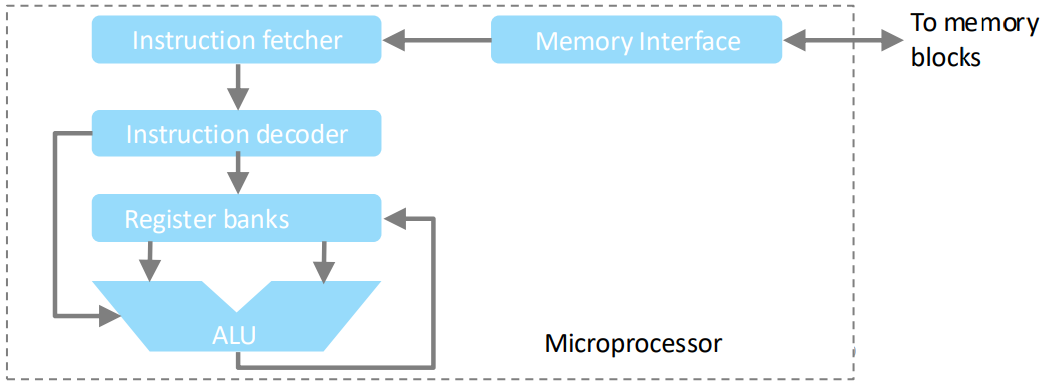
\includegraphics[width=0.8\linewidth]{img/img2.png}
    \caption{CPU schema}
\end{figure}

\paragraph{Alternative?} Field-Programmable Gate Arrays (also known as \textbf{FPGAs}), custom logic, etc. All of this things are a \textbf{dedicate hardware} that has a special purpose, indeed they are designed for a specific function. In general they use less power than CPU but they can not be used for other functions.

\paragraph{}

\textbf{Modern microprocessors} also offer features to control power consumption, via software we can reduce the consumption (sleep mode).

Microprocessor are used in combination with some custom logic for a well-defined functions, while the CPU and software is used for everything else.


\subsection{Microcontroller, MCU}

As written above, the MCU generally has a single-core processor, memory blocks, Digital and Analog I/Os and other basic pheripherals. It is typically used for a \textbf{basic control purposes}.

\begin{figure}[H]
    \centering
    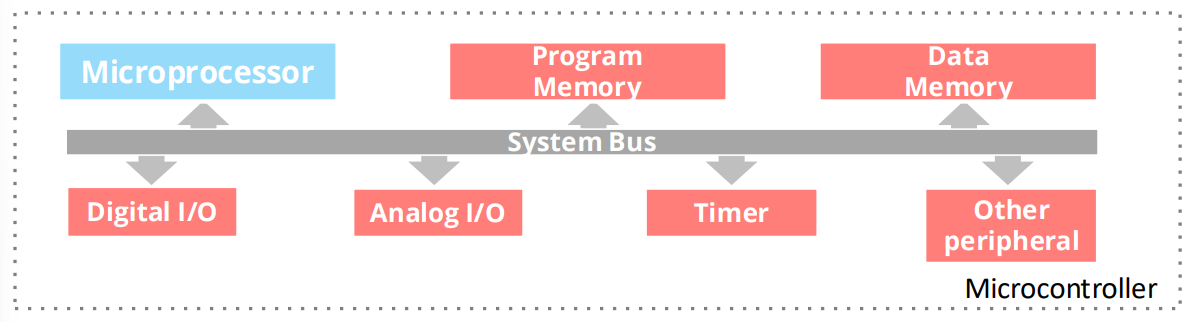
\includegraphics[width=0.8\linewidth]{img/img3.png}
    \caption{Microcontroller}
\end{figure}

\subsection{How to chose between CPUs and MCUs?}

In most embedded system, MCUs are chosen to be the best solution because they offers:

\begin{itemize}
    \item Low development and manufacturing cost;
    \item Easy porting and updating;
    \item Light footprint;
    \item Relatively low power consumption;
    \item Good performance for low-end products.
\end{itemize}

\begin{figure}[H]
    \centering
    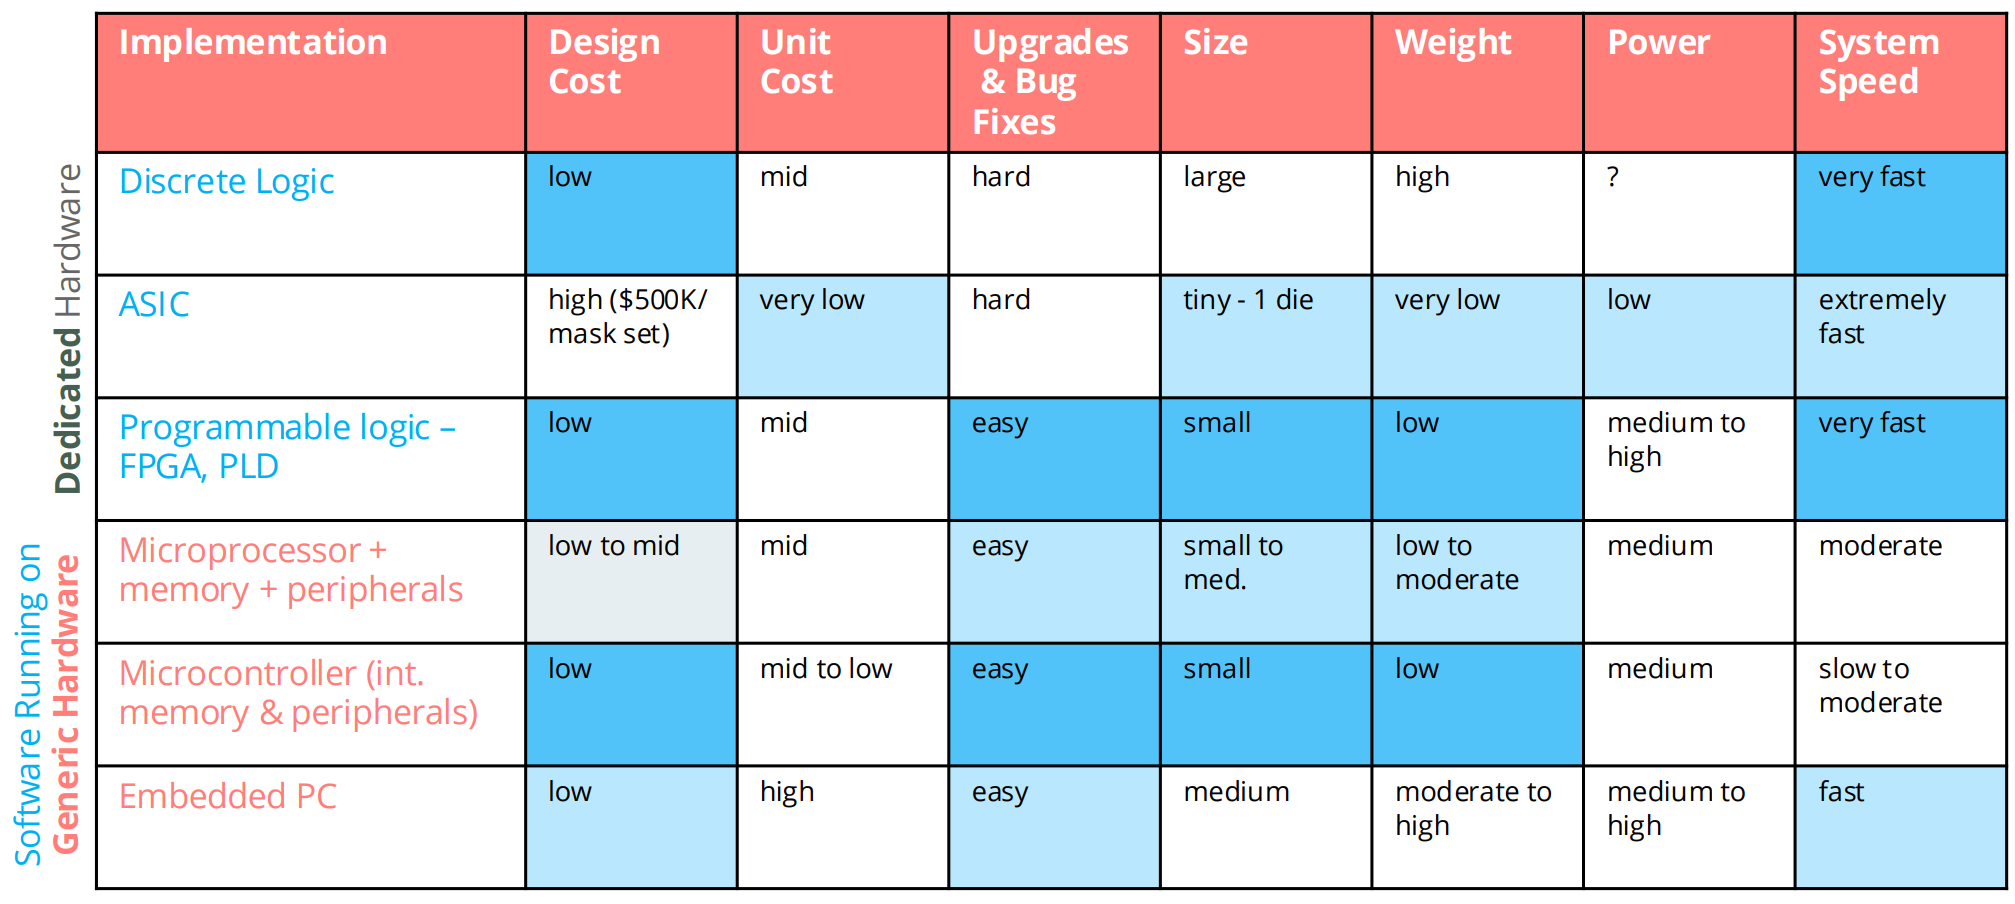
\includegraphics[width=1\linewidth]{img/img4.png}
    \caption{Options for Building Embedded Systems}
\end{figure}

Unless there's a very specific reason, such as some constraints, the best choice for embedded systems is
software running on generic hardware.


\subsection{Basic functionality of an Embedded System}

\begin{itemize}
    \item[] \textbf{Monitoring Applications: } monitor a process and adjust an output to maintain desired set point, e.g. temperature, speed...
    \item[] \textbf{Sequencing: } step through different stages, called states, based on environment and system;
    \item[] \textbf{Digital signal processing: } remove noise, select desired signal features;
    \item[]  \textbf{IoT applications: } exchange information reliably and quickly using near-by communications and networks.
\end{itemize}

\section{Challenges in Embedded System Design}

There are lots of challenges when we use the embedded system some could be: how much hardware do we need? How faster the CPU is? How do we meet our deadlines? faster HW or cleverer SW? How minimise power consumption? Turn off unnecessary logic or reduce memory accesses? How de we design for upgradeability? Is it secure?

\paragraph{}

\textbf{Testing on embedded system is complex: }we can not separate the testing of an embedded computer from the machine in witch it is embedded.
\paragraph{}
\textbf{Limited observability and controllability: }it is difficult to see how it happen, there is none screen and keyboards, we need to watch the electrical signal values.
\paragraph{}
\textbf{restricted development environments: }much more limited than those available for PCs.

\section{Attributes of Embedded Systems}

\subsubsection{Interfacing with the environment}

Analog signals from sensors, typically using a voltage value that rappresents a physical value.

\subsubsection{Concurrent and reactive behaviors: real-time constraints on responses}
Embedded systems are not single-threaded: a lot of things can happen simultaneously as they respond to
sequences and combinations of events in a timely manner.
Embedded systems typically must perform multiple separate activities concurrently, especially when
having several sensors.

\subsubsection{Fault handling}
Operate independently for long periods and handle likely faults \textbf{without crashing}


\subsubsection{Diagnostics}

Embedded systems should help developers determine problems quickly.


\subsection{Example Analog Sensor - Depth Gauge}

We want calculate how deep and underwater object is: 


\begin{itemize}
    \item[-] A sensor detects pressure and generate a proportional output voltage \textbf{Vsensor}
    \item[-] Hence an Analog to Digital converter calculate and transform the voltage into a digit 
\end{itemize}

\begin{lstlisting}[language=c++]
// Your Software
ADC_Code = adc_read();
V_sensor = ADC_code * V_ref / ADC_MASK;
Pressure_kPa = 250 * (V_sensor / V_supply + 0.04);
Depth_ft =33 * (Pressure_kPa - Atmos_Press_kPa) / 101.3;
//Actual relationship between depth and pressure
\end{lstlisting}


  \begin{minipage}{\linewidth}
      \centering
      \begin{minipage}{0.45\linewidth}
          \begin{figure}[H]
                \centering
                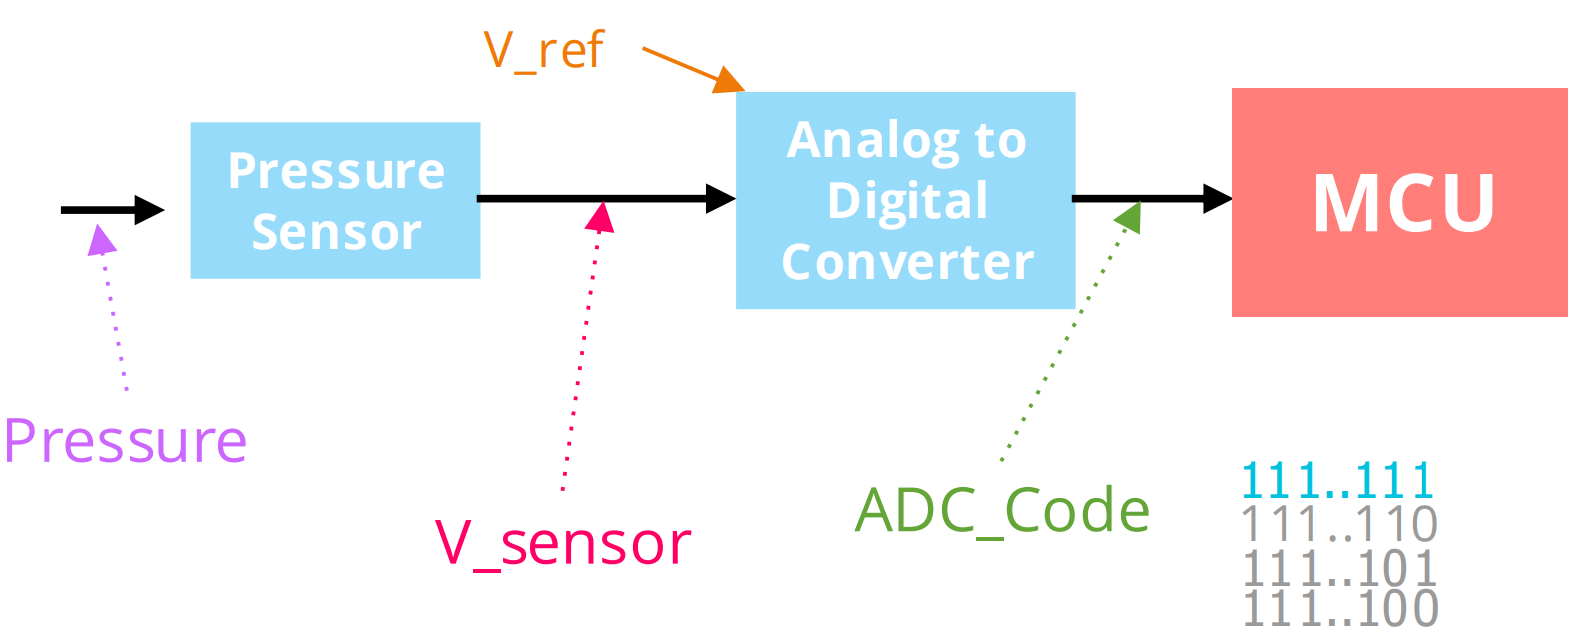
\includegraphics[width=1\linewidth]{img/img5.png}
          \end{figure}
      \end{minipage}
      \hspace{0.05\linewidth}
      \begin{minipage}{0.45\linewidth}
          \begin{figure}[H]
                \centering
                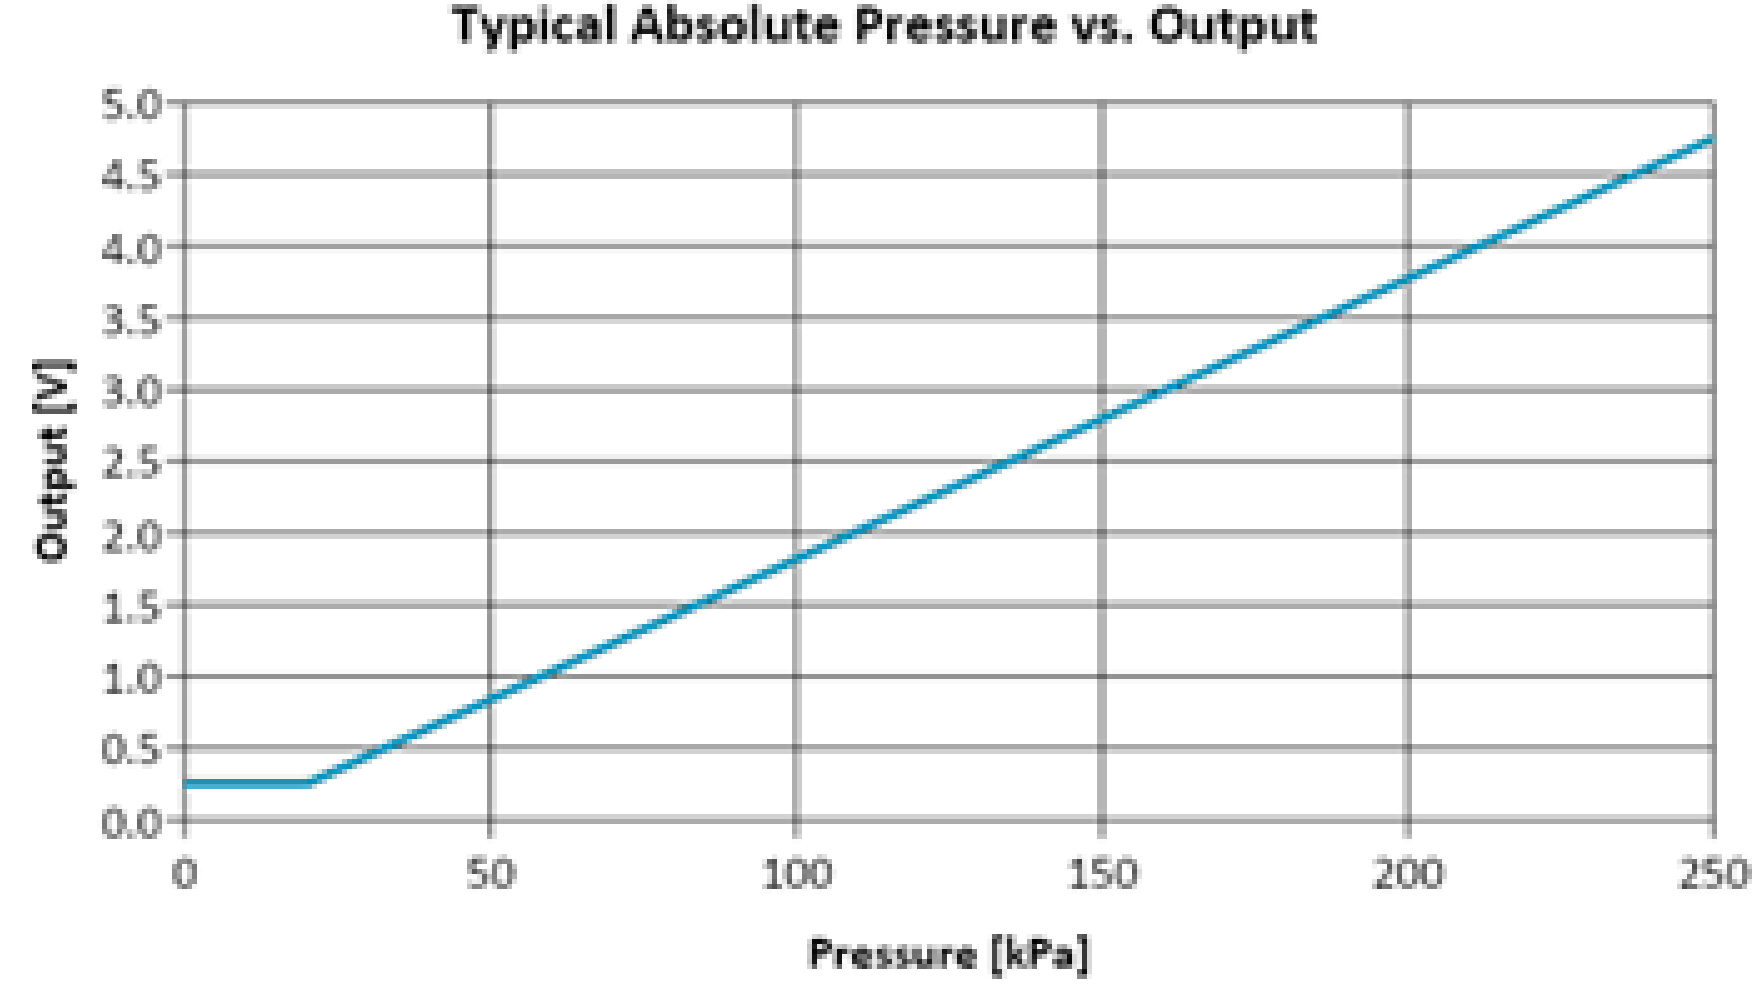
\includegraphics[width=1\linewidth]{img/image5.png}
          \end{figure}
      \end{minipage}
  \end{minipage}

\section{MCU Hardware \& Software for Concurrency}

In a microcontroller (MCU) several things happen \textbf{concurrently} while the CPU is executing instructions. 

Specialized hardware peripherals add dedicated \textbf{concurrent processing}, like analog interfacing, timers,
and detecting external signal events. Peripherals use interrupts to notify the CPU of events.

Embedded systems rely on both MCU hardware peripherals and software to get everything done concurrently on time


  \begin{minipage}{\linewidth}
      \centering
      \begin{minipage}{0.25\linewidth}
          \begin{figure}[H]
                \centering
                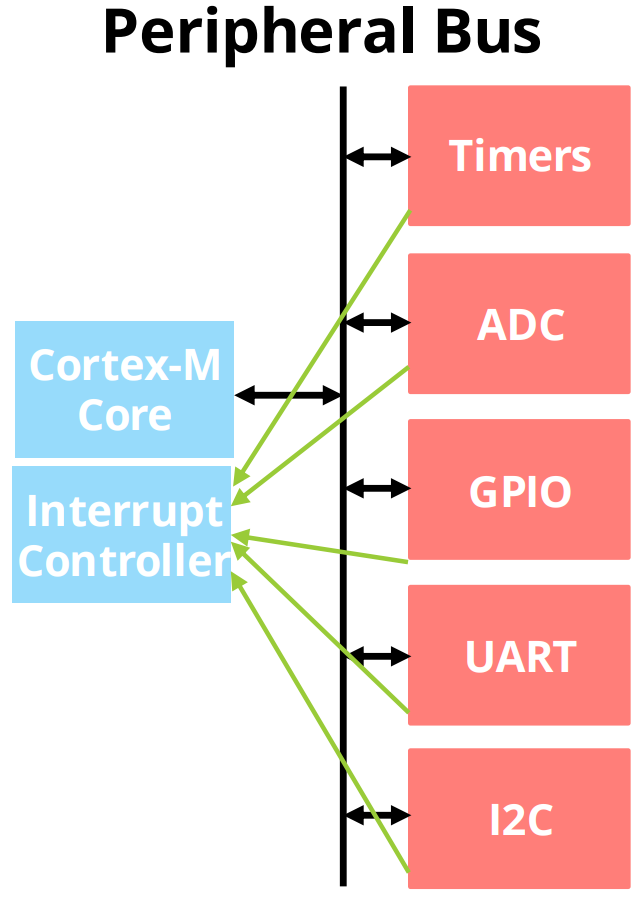
\includegraphics[width=1\linewidth]{img/image6.png}
          \end{figure}
      \end{minipage}
      \hspace{0.05\linewidth}
      \begin{minipage}{0.65\linewidth}
          \begin{figure}[H]
                \centering
                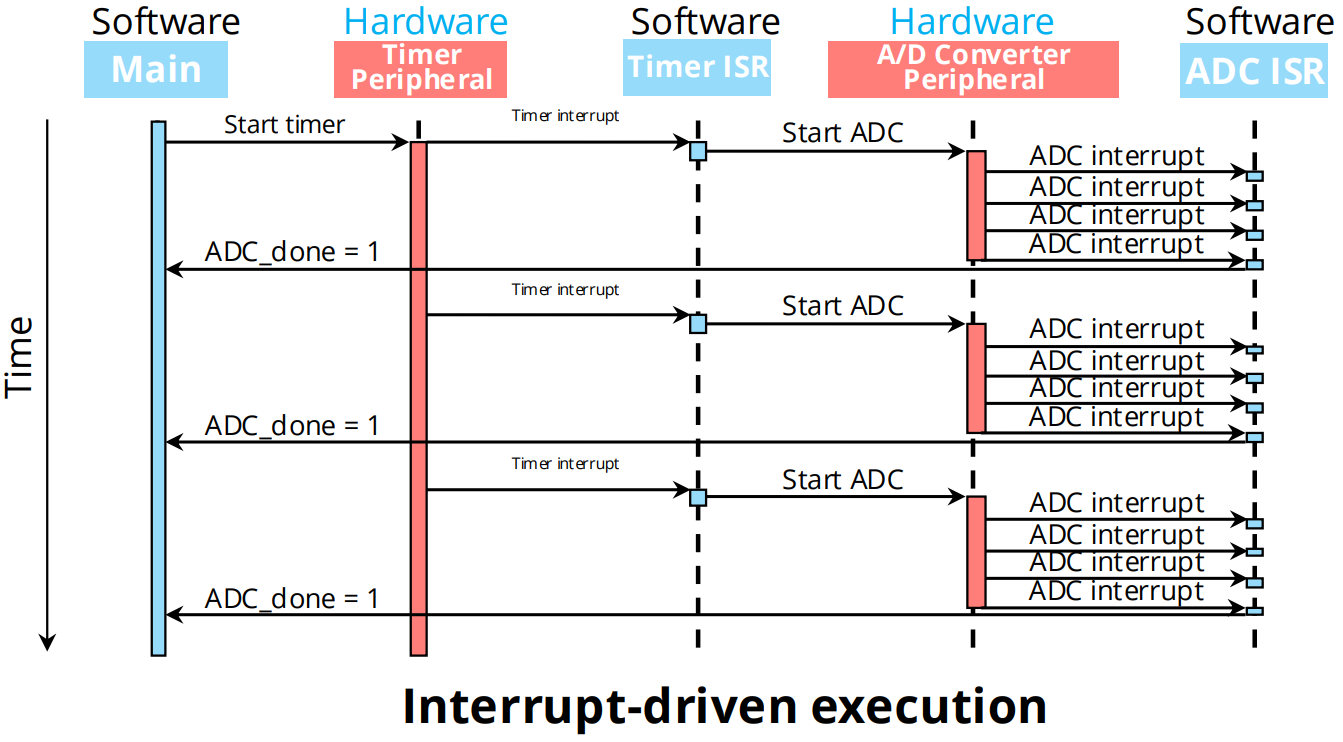
\includegraphics[width=1\linewidth]{img/image7.png}
          \end{figure}
      \end{minipage}
  \end{minipage}


\subsection{Embedded Software}

Programmed in C rather than Java (smaller and faster code, so less expensive MCU). Some performance-critical code may be in \textbf{assembly language}.

Typically, no OS, but instead a simple scheduler (or even just interrupts + main
code (foreground/background system). If OS is used, likely to be a lean \textbf{RTOS}


\subsection{Hardware and Software Co-design Model}

Commonly both the hardware and the software for embedded system are \textbf{developed in parallel}, this allow to optimize the overall
product's design, functionality and manufacturing/development cost.

Push things to the software layer if functionality can be achieved in software, this reduce  the  overall hardware \textbf{complexity} and cost.

\subsection{Functional vs. Non-functional Requirements}

Embedded systems have \textbf{MANY non-functional requirements} (how the system should perform). Timing
correctness is way more critical in embedded systems, especially in medical, transportation and
military systems.

Non-functional requirements can be: the time required to compute an output, the system's size, weight,
portability, power consumption, battery capacity, reliability and so on.


\paragraph{}
\textbf{Functional requirements are user-centric}, tangible and observable, and specify what the system must do.

\newpage
\section{Internet of Things (IoT)}
An Internet-of-Things system is a networked embedded
computing system. An IoT system is addressable
via a network.

Some examples are smart buildings and home appliances, wearable devices, medical devices.

\paragraph{}
Networking is a \textbf{critical component} of an IoT system

\subsection{Why IoT?}
\begin{itemize}
    \item[] Items can have more functionality and become more intelligent
    \item[] Items can be managed more easily
    \item[] More information becomes available
\end{itemize}


\subsection{Cyber-physical Systems}

Combines physical devices with computers that control the device. The embedded computer is the cyber part that replaces mechanical controllers:

\begin{itemize}
    \item more accurate and more sophisticated control
    \item monitors and controls the physical processes with feedback loops
\end{itemize}

\begin{figure}[H]
    \centering
    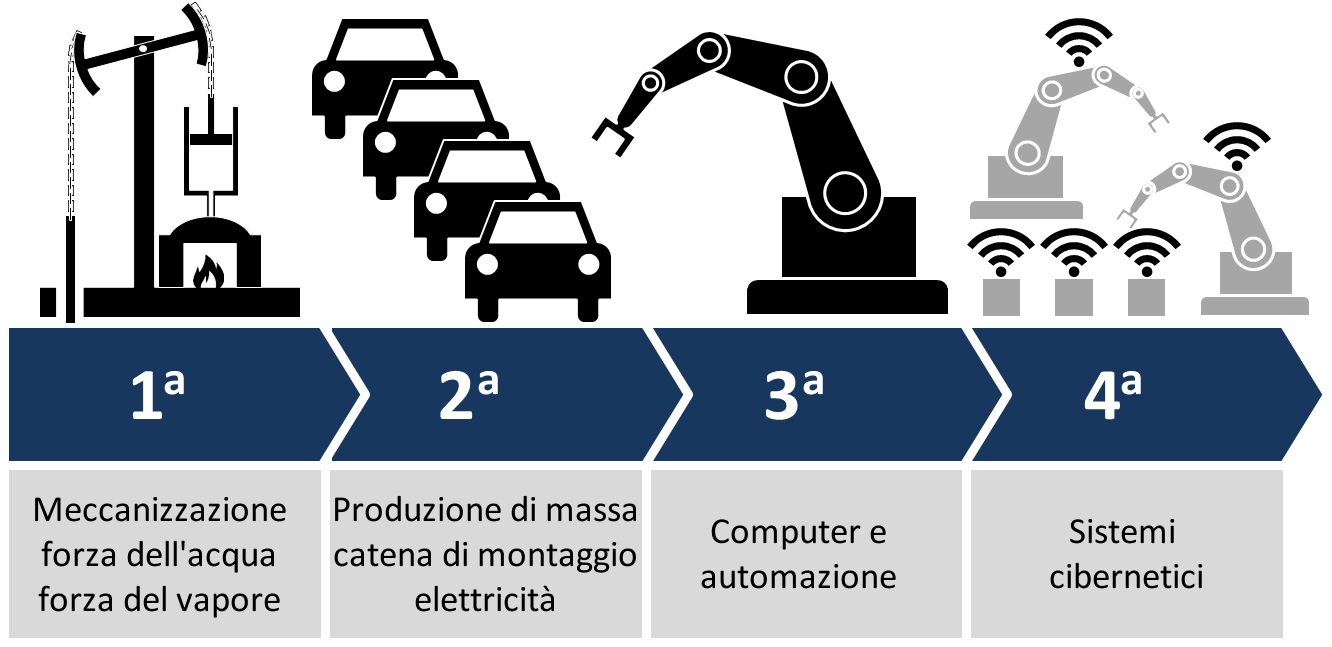
\includegraphics[width=0.5\linewidth]{img/Industry_4.0_ita.png}
\end{figure}

\section{Summary}

An embedded system is built for a specific application. It has complex hardware and software components.


Embedded systems pose many design challenges: Functional, output as a function of input, and non-functional requirements, Deadlines, power, cost.

In real-time systems, \textbf{timing correctness} is just as important as functional
or logical correctness